% Solution: Munoz-Garcia & Toro-Gonzalez (2019) Ch. 4 Exercise 3 "Sequential Version of the
% Prisoner's Dilemma Game". Input by \solitem.
% Reused from lista-reais-lectures-01-04-solutions/item14.tex, deepened (full normal form, all
% Nash equilibria including mixed ones). Check: check_B_L03.py.
\begin{exsol}{\MG{} Ch.~4, Exercise 3}{160}{Foundations}{1}
\asked In the sequential prisoner's dilemma of Fig.~4.9: (a) player~2's best reply to each
move of player~1; (b) player~1's move and the subgame-perfect equilibrium; (c) whether play
differs from the simultaneous version (Ch.~1, Fig.~1.8).

\method Backward induction in a finite game of perfect information (Lecture~3, slide~30;
Tadelis \S8.1, Prop.~8.1, p.~153); in such games the SPE are exactly the backward-induction
profiles (Lecture~3, slide~35). An SPE is written as complete strategies: player~2's strategy
names a reply at \emph{both} of her nodes, including the one off the path (Lecture~3, slide~25;
Tadelis Def.~7.4, p.~138; Gibbons pp.~125--126 on outcome vs.\ equilibrium). All Nash equilibria
of the normal form are found with the best-reply and indifference conditions (principle of
indifference, Lecture~3, slides~10--12).

\solution
\textbf{Notation.} $C$ = Confess, $N$ = Not confess. Payoffs $(u_1,u_2)$ from Fig.~4.9:
$(C,C)\mapsto(-5,-5)$, $(C,N)\mapsto(0,-15)$, $(N,C)\mapsto(-15,0)$, $(N,N)\mapsto(-1,-1)$.
Player~2's strategy is a pair $s_2 = s_2(C)\,s_2(N)$: her reply after $C$, then after $N$. So
$S_2 = \{CC, CN, NC, NN\}$ and $S_1 = \{C, N\}$.
\begin{center}
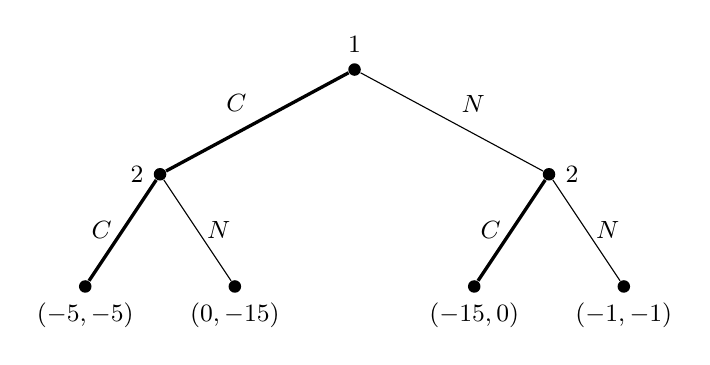
\begin{tikzpicture}[scale=0.95,dot/.style={circle,fill,inner sep=1.6pt},
  every node/.style={font=\small}]
  \node[dot,label=above:{1}] (r) at (0,0) {};
  \node[dot,label=left:{2}] (a) at (-2.6,-1.4) {};
  \node[dot,label=right:{2}] (b) at (2.6,-1.4) {};
  \draw[very thick] (r) -- node[above left] {$C$} (a);
  \draw (r) -- node[above right] {$N$} (b);
  \node[dot,label=below:{$(-5,-5)$}] (aa) at (-3.6,-2.9) {};
  \node[dot,label=below:{$(0,-15)$}] (ab) at (-1.6,-2.9) {};
  \node[dot,label=below:{$(-15,0)$}] (ba) at (1.6,-2.9) {};
  \node[dot,label=below:{$(-1,-1)$}] (bb) at (3.6,-2.9) {};
  \draw[very thick] (a) -- node[left] {$C$} (aa);
  \draw (a) -- node[right] {$N$} (ab);
  \draw[very thick] (b) -- node[left] {$C$} (ba);
  \draw (b) -- node[right] {$N$} (bb);
\end{tikzpicture}\\[2pt]
{\footnotesize Fig.~4.9 redrawn; thick branches = backward-induction choices.}
\end{center}

\textbf{(a) Player 2's best replies.}
\begin{align*}
  \text{after } C:&\quad u_2(C,C) = -5 > -15 = u_2(C,N) \ \Rightarrow\ C;\\
  \text{after } N:&\quad u_2(N,C) = 0 > -1 = u_2(N,N) \ \Rightarrow\ C .
\end{align*}
So $s_2^* = CC$: confess whatever player~1 did.

\textbf{(b) Player 1's move and the SPE.} Replacing each of player~2's nodes by its outcome,
\[
  u_1(C, s_2^*) = u_1(C,C) = -5 \;>\; -15 = u_1(N,C) = u_1(N, s_2^*),
\]
so player~1 confesses. The SPE is
\[
  (s_1^*, s_2^*) = \bigl(C,\ (C \text{ after } C,\ C \text{ after } N)\bigr) = (C, CC),
\]
with outcome $(C,C)$ and payoffs $(-5,-5)$. It is unique: every comparison above is strict.

\textbf{Normal form and all Nash equilibria (deepening).}
\begin{center}
\begin{tabular}{r|c|c|c|c|}
\multicolumn{1}{r}{} & \multicolumn{1}{c}{$CC$} & \multicolumn{1}{c}{$CN$} &
\multicolumn{1}{c}{$NC$} & \multicolumn{1}{c}{$NN$}\\ \cline{2-5}
$C$ & $\br{-5},\ \br{-5}$ & $-5,\ \br{-5}$ & $\br{0},\ -15$ & $\br{0},\ -15$ \\ \cline{2-5}
$N$ & $-15,\ \br{0}$ & $\br{-1},\ -1$ & $-15,\ \br{0}$ & $-1,\ -1$ \\ \cline{2-5}
\end{tabular}
\end{center}
Underlined payoffs are best replies. \emph{Pure:} only $(C, CC)$ has both payoffs underlined.
\emph{Mixed:} let $p = \Pr_1(C)$.
\begin{itemize}
  \item If $0 < p < 1$, player~2's payoffs are $-5p$ ($CC$), $-5p - (1-p)$ ($CN$), $-15p$ ($NC$),
  $-15p - (1-p)$ ($NN$); $CC$ is the unique best reply, and against $CC$ player~1 strictly prefers
  $C$ ($-5 > -15$), so $p = 1$. Contradiction.
  \item If $p = 0$, player~2's best replies are $CC$ and $NC$ (both reply $C$ to $N$), and against
  either one $C$ pays player~1 $-5$ or $0$, more than $-15$. Contradiction.
  \item If $p = 1$, player~2's best replies are $CC$ and $CN$ (both reply $C$ to $C$; they differ only
  at the unreached node). Let $w = \Pr_2(CN)$. Player~1 keeps $C$ iff
  \[
    u_1(C) = -5 \;\ge\; u_1(N) = -15(1-w) + (-1)w = -15 + 14w \iff w \le \tfrac{5}{7}.
  \]
\end{itemize}
So the Nash equilibria are $\{(C,\ (1-w)\,CC + w\,CN) : 0 \le w \le \frac57\}$, all with outcome
$(C,C)$. Only $w = 0$ is subgame perfect: for $w > 0$ player~2 plans $N$ after $N$ with positive
probability, which is not a best reply in that subgame ($-1 < 0$). In behavioral terms: player~2
plays $C$ after $C$ and, after $N$, plays $N$ with probability at most $\frac57$.

\textbf{(c) Comparison.} In the simultaneous game (Fig.~1.8) $C$ is strictly dominant for each
prisoner ($-5 > -15$ and $0 > -1$), so the unique Nash equilibrium is $(C,C)$ with $(-5,-5)$. The
sequential version has the same outcome. Seeing player~1's move does not change player~2's
choice, because $C$ is her best reply to each of player~1's moves; player~1 therefore gains
nothing from moving first.

\interp Observing the other's move matters only when the best reply depends on it. Here it does
not: confessing is dominant at both of player~2's nodes, so the sequential game unravels exactly
as the simultaneous one, and the Pareto-better $(N,N)$ is still out of reach. The mixed Nash
equilibria show what subgame perfection removes even here: a ``promise'' by player~2 to
reciprocate silence ($N$ after $N$) is cheap talk once player~1 has stayed silent, the Lecture~4
lesson that talk is cheap unless something makes it credible (Lecture~4, slide~11). Moving first
is a commitment device only when it changes what the follower wants to do (Stackelberg,
Lecture~3, slide~37).

\verify \texttt{check\_B\_L03.py} runs backward induction on the tree (unique result: path
$C$, $C$ with payoffs $(-5,-5)$), finds the pure Nash equilibria of the $2\times4$ normal form (only
$(C, CC)$) and of the simultaneous game (only $(C,C)$), confirms on a grid of $w$ in steps of
$\frac1{70}$ that $(C, (1-w)CC + wCN)$ is a Nash equilibrium exactly when $w \le \frac57$, and that
no Nash equilibrium puts weight on $N$. Output line: \texttt{munoz-garcia-4-3: SPE (C, CC); NE =
(C, CC with prob >= 2/7)}. \emph{Comparison with \MG{}'s answer} (pp.~160--162): it agrees on all
three parts, $\text{SPNE} = \{(\text{Confess}, \text{Confess}, \text{Confess})\}$. One wording slip
there: the third component is described as player~2's response ``to player~1 selecting Confess (in
Subgame~3)''; Subgame~3 follows Not Confess, so it is the reply to Not Confess. The book does not
list the mixed Nash equilibria.

\mistakes
\begin{itemize}
  \item Writing the SPE as the outcome $(C, C)$: player~2's strategy must say what she does after
  $N$ too, so the SPE is $(C, CC)$.
  \item Concluding that the sequential game has a different equilibrium because ``player~2 can
  punish''. Punishment after $N$ is not a best reply, so it is not part of any SPE.
  \item Claiming that $(C, CC)$ is the only Nash equilibrium: it is the only \emph{pure} one, but
  player~2 may mix off the path ($w \le \frac57$).
\end{itemize}

\answer{(a) Player~2 confesses after Confess ($-5 > -15$) and after Not confess ($0 > -1$).
(b) Player~1 confesses ($-5 > -15$); SPE $= (C, (C, C))$, outcome $(C,C)$, payoffs $(-5,-5)$.
Nash equilibria: $(C,\ (1-w)CC + wCN)$, $0 \le w \le \frac57$; only $w = 0$ is subgame perfect.
(c) No difference: the simultaneous game's unique equilibrium is also $(C,C)$, since Confess is
strictly dominant at every node.}
\end{exsol}
